\documentclass[sigconf]{acmart}

\usepackage{booktabs} % For formal tables


% Copyright
%\setcopyright{none}
%\setcopyright{acmcopyright}
%\setcopyright{acmlicensed}
%\setcopyright{rightsretained}
%\setcopyright{usgov}
%\setcopyright{usgovmixed}
%\setcopyright{cagov}
%\setcopyright{cagovmixed}


% DOI
\acmDOI{10.475/123_4}

% ISBN
\acmISBN{123-4567-24-567/08/06}

%Conference
\acmConference[MMSys'17]{ACM Multimedia Systems}{June 2017}{Taipei, Taiwan} 
\acmYear{2017}
\copyrightyear{2017}

\acmPrice{15.00}


\begin{document}
\title{The use of Human Power on Video Synchronization}


\author{Removed for Blind Review}


% The default list of authors is too long for headers}
\renewcommand{\shortauthors}{Removed for Blind Review}


\begin{abstract}
User Generated Videos are contents created by heterogeneous users around an event. Each user films the event with his point of view, and according to his limitations. In this scenario, it is impossible to guarantee that all the videos will be stable, focused on a point of the event or other characteristics that turn the automatic video synchronization process possible. Focused on this scenario we propose the use of crowdsourcing techniques in video synchronization (CrowdSync). The crowd is not affected by heterogeneous videos as the automatic processes are, so it is possible to use them to process videos and find the synchronization points.  In order to make this process possible, a structure is described that can manage both crowd and video synchronization: the Dynamic Alignment List (DAL). Therefore, we carried out three experiments to verify that the crowd can perform the proposed approach: the first experiment used a crowd simulator to verify the DAL capability of managing videos and contributions, generating cohesive video presentations; the second experiment used a crowd to synchronize videos performing small tasks; the third explored the use of the crowd to synchronize Live Stream Videos, through the development of the LiveSync tool.
\end{abstract}

%
% The code below should be generated by the tool at
% http://dl.acm.org/ccs.cfm
% Please copy and paste the code instead of the example below. 
%
\begin{CCSXML}
<ccs2012>
<concept>
<concept_id>10002951.10003227.10003251</concept_id>
<concept_desc>Information systems~Multimedia information systems</concept_desc>
<concept_significance>300</concept_significance>
</concept>
<concept>
<concept_id>10003120.10003130</concept_id>
<concept_desc>Human-centered computing~Collaborative and social computing</concept_desc>
<concept_significance>300</concept_significance>
</concept>
</ccs2012>
\end{CCSXML}

\ccsdesc[300]{Information systems~Multimedia information systems}
\ccsdesc[300]{Human-centered computing~Collaborative and social computing}

% We no longer use \terms command
%\terms{Theory}

\keywords{Synchronization, Video, Crowdsourcing}

\maketitle


\section{Introduction}
\label{sec:intro}
Nowadays users don't need to rent fancy and expensive devices, neither depended on professionals to produce and share video, they can with their mobiles create User Generated Video (UGV). UGV is a kind of multimedia content created by heterogeneous users, shared online and without any explicit coordination mechanism. UGVs can be grouped around an event: a particular geographical space shared by a group of people at a particular period of time, such as protests, music festivals or sport games, resulting in awesome enahnced contents that can be reused in many ways. Moreover, each one of these videos reveals a unique point of view about what is happening, according to the user's identity and beliefs (in terms of ideology, team and group identification etc.) as well as user's context and preferences (in terms of positioning, device capabilities and limitations etc.). 

In this scenario, it is impossible to ensure that all the UGV related to a same significant moment in a social event will be stable, have similar visual and aural quality or even if this moment was captured by the user. Then, automatic video synchronization techniques are not so effective. The synchronization of UVG about a particular topic or event can be announced as storytelling problem. Intuitively, this problem can also viewed as a synchronization problem, in which all of the related contents must be, firstly, positioned in a same global timeline and, in the sequence, arranged to produce a coherent narrative flowing.

Focused on this scenario, this paper introduces the idea of using crowdsourcing techniques for UGV synchronization, once the human processing is less affected by the heterogeneity of UGV content. Hence, we claim that the process of finding the synchronization points between UVG should involve crowd workers when automatic techniques are not effective. Also, the announced synchronization problem must consider many issues and in this paper, we focus on a particular issue: how to manage both crowd and video synchronization information and use them to rebuild the story of an event. In this sense, the paper introduces the Dynamic Alignment List (DAL), a data structure to assist the crowd contributions process as well as the generation of a coherent presentation of an event using UVG content. 

We conducted three experiments to to investigate if the crowd would perform the proposed approach: the first used a crowd simulator to verify the DAL capability of managing videos and contributions, generating coherent presentations from user generated videos; the second experiment used a crowd to synchronize videos performing small tasks. The LiveSync Tool, developed to test if the crowd can be used to synchronize live streaming events, is detailed and shows how to use the structure to synchronize live strems. Last but not least, the focus of the paper is to show that the crowd can be used in scenarios where automatic techniques may find challenges, not to state that the use of the crowd is better than the automatic techniques.

%Trabalhos relacionados






\subsection{Chunk Synchronization}
\label{chunk-sync}
Following the crowdsourcing approach, we can't let each crowdworker analyse all the entire videos to find all synchronization points. This would require too much effort of each crowdworker. For the current version of our CrowdSync system, we split the videos in small chunks of 5s each. This way we make each task a lot easier to each crowd member, because for each task he needs only to compare if two chunks overlaps and if they do, what is the $\Delta$ that makes them synchronous.

Figure~\ref{chunks_process} shows this synchronization method. First each video A e B is mapped in chunks of 5s. A pair of chunks is sent to a crowdworker that evaluates if there is synchronization and what is the $\Delta$ if there is any. In the example (Figure~\ref{chunks_process}), if the chunks [$C_{1}A$,$C_{1}B$] have no synchronization, we compare the next possibility [$C_{1}A$,$C_{2}B$] and so on until we find it or we compare all chunks. In the example the pair [$C_{1}A$,$C_{3}B$] contains a synchronization point. The crowdworker identifies it and discovers the time offset between them ($\Delta$). Using the value of $\Delta$ and knowing which chunks where the ones where the synchronization point was found, we can synchronize the full videos [A,B]. In the example, the final difference between the two videos [A,B] is $\Delta$ plus two times the chunk size, because $\Delta$ was found in the relation between the first chunk of A and the third of B, a difference of two chunks.

\begin{figure}[h]
	\centerline{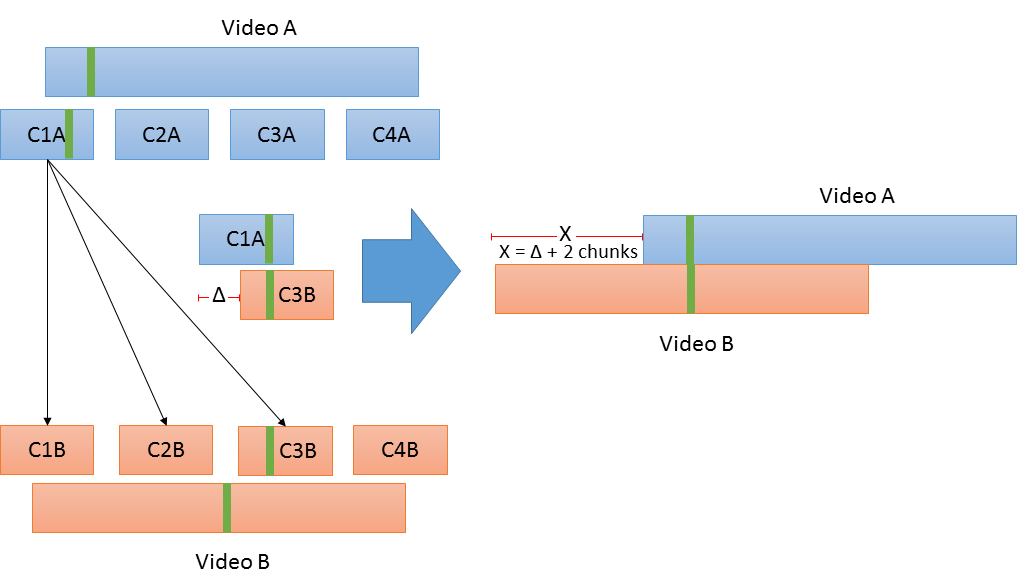
\includegraphics[scale=0.35] {figure/chunks}}
	\caption{Chunk Synchronization Method}
	\label{chunks_process}
\end{figure}

When two chunks associated with two videos are synchronized, all the contents of these two videos will also be synchronized. This happens because as described in the introduction, we consider the videos as continuous. And if comparing all chunks from both videos, we can't find any synchronization point, those two probably have no synchronization point. We say probably, because there is a possibility that the crowd fails in its tasks. To reduce this possibility, there are measures that can be taken such as assessing the crowd for better contributions. We however do not discuss this issue in this paper, as our scope focus on the synchronization process only. Another important consideration here is that this approach can fall in the worst case when there is no synchronization point, and all chunks will be compared, and will fail. On the other hand, if there is an synchronization point, we can find it in the first comparison.

\subsection{Frame Synchronization}
\label{frame-sync}
The Frame synchronization is an enhancement proposal on top of the chunk model. Here, instead of using video chunks, each crowdworker receives the key-frames sequences from two videos that must be synchronized. This way, each worker has access to the full video at once, enhancing the possibilities of finding a synchronization point. However, as now the worker interacts with frames, if a pair of frames is identified as a possible synchronization point, its precision is reduced, making necessary a second step on the task: watch the videos based on the information provided by the two frames (each frame has a timestamp from when it which part of the video it was removed, making possible to calculate $\Delta$ such as in the chunk based one).

Figure~\ref{frames} shows the interface developed to this approach: on the top the user selects the probably aligned frames (or close ones) and plays the videos. If it is correct, he confirms the alignment, else he tries again or discard the synchronization. 

\begin{figure}[h]
	\centerline{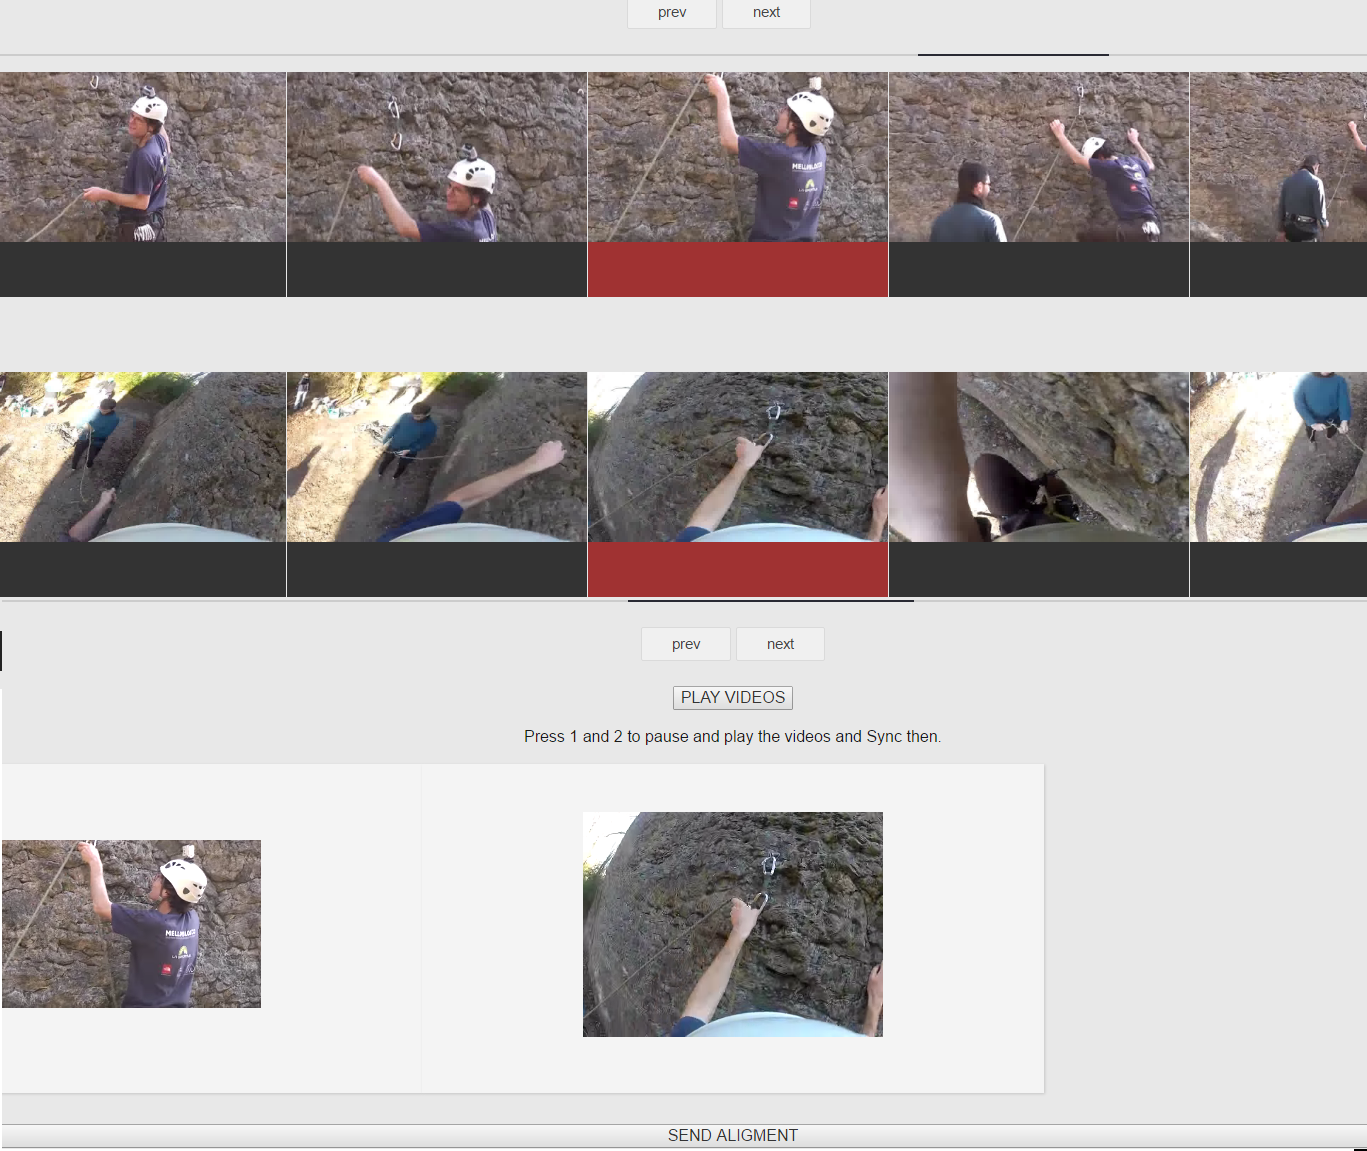
\includegraphics[scale=0.25] {figure/frames}}
	\caption{Frame Synchronization Method}
	\label{frames}
\end{figure}






\subsection{LiveSync}



\section{Dynamic Alignment List}
Besides the synchronization method, there is the need to manage all the generated tasks: which pair of chunks will be sent to each user? From which videos? Where are the contributions stored? How can the contributions be validated? How to know that all videos are synchronized? What are the time offsets among the videos? Do I need to compare all videos?

Trying to answer these questions, we developed the concept of a  Dynamic Alignment List. It is responsible for managing all contributions, checking the convergence of the contributions, distributing the videos, inferring unknown values and storing $\Delta$ values for each pair of videos.

The DAL has two main features: (i) time offset and (ii) contribution managements. The time offset management deals with all videos relations manipulation while the contributions management takes care of the crowd management.

\subsection{Structure}
The DAL isn't just a list as the name may suggests, it is a data structure composed of vectors and lists that are used to assist the processing of contributions of crowd workers as well as to support the generation of presentations with the synchronized videos. It was designed in order to efficiently store all relevant contributions that represent a temporal relation between a pair of videos.

Its structure is based on a Upper Triangular Matrix, although, the DAL is constructed on demand, saving space because it doesn't have any empty slot on it, turning it into a dynamic structure. In Figure~\ref{structure-dal} it is shown an instance of a DAL with five videos and its relations.

\begin{figure}[h]
	\centerline{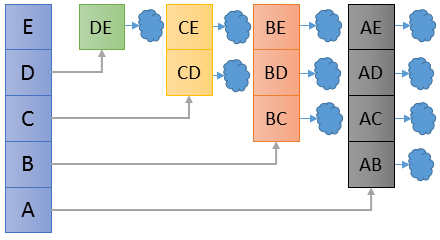
\includegraphics[scale=0.7] {figures/DAL/dal}}
	\caption{DAL Structure}
	\label{structure-dal}
\end{figure}

The DAL starts as an array that contains in its positions the videos that are going to be related (blue squares). Each video is an object that contains a reference to the media that it represents (URI) or other DAL (creating a hierarchy), a reference to the array of relations with the other videos and an attribute with the duration ($\sigma$) of the video.

These relations are cells into an array. Each position of this array is a different relation that represents the time offset between those two videos. Each position of the array stores the IDs for the pairs of videos that are being related, an attribute that contains the current $\Delta$ (time offset), an attribute that contains the degree of confidence in that relation and a list of contributions on that relation (each contribution on which is the $\Delta$ value). The degree of confidence is how precise the current $\Delta$ is believed to be true. Note that we don't need to store all direct relations (e.g. $\Delta_{A,H}$ and $\Delta_{H,A}$), we can store one direct relation and its complementary can be easily calculated ($\Delta_{A,H} = -\Delta_{H,A}$).

A contribution (in the blue cloud) in turn has the $\Delta$ proposed by each user for that relation and a reference for that user (the user profile may be used to rise the degree of confidence of a relation).

\subsection{Time Offset Management}
The first feature (and original purpose) of the DAL is the Time Offset Management. It is responsible for dealing with all aspects of the time offset relation among videos. These aspects are:

	\textbf{$\Delta$ Storage and Retrieval:} a characteristic of the DAL is to allow the addition, update and retrieval of any Time Offset for any pair of videos. This gave us the starting point of using a Matrix like structure that permits fast access to any cell of the matrix  from a pair of coordinates. This way knowing the two videos which we desire to know or to update the $\Delta$, we can quickly obtain this information. However we don't use a pure matrix for two main reasons: information redundancy, we don't need to store the AB and BA relations, as one is the opposite of the other ($\Delta_{i,j} = -\Delta_{j,i}$, eq.~\ref{eq-oposite}); and a matrix doesn't allow the storage of multiple contributions in the same cell (requisite for the crowdsourcing);
\begin{eqnarray}
	\label{eq-oposite}
	\Delta_{i,j} = b.i - b.j	\nonumber \\
	\Delta_{j,i} = b.j - b.i	\nonumber \\
	-\Delta_{j,i} = b.i + b.j	\nonumber \\
	\Delta_{i,j} = -\Delta_{j,i}
\end{eqnarray}

	\textbf{$\Delta$ Inference:} known relations in the DAL allows developing inference methods that use transitivity through pairs of aligned videos to calculate relations between videos,in which the offset is still unknown. If we know the relation AB and AC from the structure we can infer BC.	
\begin{eqnarray}
	\label{dina-i}
	\Delta_{B,C} = b.B - b.C	\nonumber \\
	\Delta_{B,A} = b.B - b.A \rightarrow b.B = \Delta_{B,A} + b.A	\nonumber \\
	\Delta_{A,C} = b.A - b.C \rightarrow b.A = \Delta_{A,C} + b.C	\nonumber \\
	\Delta_{B,C}= \Delta_{B,A} + b.A - (b.A-\Delta_{A,C}) \rightarrow \nonumber \\ \Delta_{B,C} = \Delta_{B,A} + \Delta_{A,C}	
\end{eqnarray}

	\textbf{Presentation Generation:} With the known and inferred time offsets, it is possible to create a presentation of the event that correlates all videos with temporal relations. This presentation can be the maximal one, where the event is presented using the first video until the end of the last one, also when videos with overlapping exists, the option to change camera is made available to users.

\subsection{Contribution Management}
The Contribution Management is a requisite in order to adequate the DAL for a crowdsourced scenario. It is necessary to receive, distribute and process the crowd contributions in order to find the correct Time Offsets. The aspects involved in the Contribution Management are:

	\textbf{Convergence:} one of the principles of crowdsourcing is collecting the contribution of multiple members and based on these contributions finding the solution to a problem. In our case, the crowd watches the videos fragments and find synchronization points. The convergence is responsible for getting all theses contribution, and merging them in actual results.
	
	The Convergence Level detects the tendency of the Crowd about the Relation of a pair of videos. This tendency is an indicative of the agreement on a Delta between the videos. According to the scenario, a Convergence Threshold that is used to determine if a Relation is converged, is defined. Each Relation have an attribute that stores its current convergence level. If this level reaches a Convergence Threshold the method returns True, otherwise it returns False.

	Initially all Relations are created with Convergence Level 0, and consecutive similar contributions increase this value. If a tendency change in the contributions is detected, the Convergence Level is reset.
	
	\textbf{Video Selection:} the convergence deals with the problem of receiving and processing the crowd contributions. However, we must correctly choose the videos to be evaluated by the crowd that results in a contribution. The selection of these videos is part of the contribution management. 
	
	This method intent is to select which pair of videos should have priority to receive contributions. It consists of a sequence of two other methods: (i) Choose the next Video; (ii) Choose the next Relation. When this method returns NULL, it means that the DAL has been converged.
	
In order to increase possible inferences over the contributions, the method try to spread contributions over the timeline, proceeding a random selection among the Videos that were not converged nor marked as a Impossible relation. Once a Video is chosen the method select from its Relations array the Relation closer to converge.

\section{Experiments}
Aiming to verify the CrowdSync method and the data structure generated to implement the method, two different experiments were executed:

\begin{description}
	\item[LiveSync Tool:] the LiveSync Tool implements all requisites for live synchronizing live UGV streams. Its objective is to allow the creation of mash applications of related video streams with client based solutions.
	\item[Crowd Simulated DAL:] the second experiment uses a simulated crowd to verify the DAL. The objective here is to verify if the DAL correctly stores, infers, converges and selects videos and relations. We simulate the crowd so we can make a controlled analysis in a set of videos with different crowd profiles.
	\item[UGV Dataset Synchronization:] in the third experiment, real users (crowd workers) synchronize a user generated video dataset using a developed platform with all characteristics described in this paper. Since the simulated experiment allows only to verify the correct functioning of the algorithms and structure, the focus here is to verify if humans using their perception can find the synchronization points in all related videos.
\end{description}

\subsection{LiveSync Tool}
\label{livesync}
The main functionalities provided by our tool are:

\textbf{Synchronized Live Video Player:} The tool permits users to watch multiple videos synchronized. He selects from a list of sources the videos he wishes to watch and them they are synchronized using information provided by other users. If a pair of videos does not have any information about their synchronization, users are invited to contribute and synchronize the videos.

\textbf{Synchronization Infering:} In some cases that there is no direct information about the synchronization of two videos, the tool is able to infer the synchronization about them, based on the contributions of other videos. We use the transitive attribute of video synchronizations, where if we know AB and BC synchronization info (couplers), we can infer AC. To infer this value we travel trough the DAL, finding the unknown relations (for example, CE), and try to find a path of known relations where we can infer CE. Taking the DAL in Figure 1, we can infer CE if we know: AC and AE. This a two steps route, but we try all possible routes when inferring, in a way that we fill as much relations as possible.

\textbf{Video Aggregation:} Although the focus of the LiveSync tool is on synchronization, we allow users to add new stream sources to the application. He only needs to set the video source, and the video will be added to the DAL and list of videos. However, we don't do any filtering about the added video, this means that the user can add any video to the application, even ones that contains none relation with the other videos. In future versions we plan to add options where other users can mark the video as not related, and then remove them.

\textbf{Multiple Video Platform Support:} One keypoint of our tool is the use of other platforms as video sources. The videos that we play to users and that are synchronized, are not provided by us, but by other live video stream platforms. To be compatible with our tool, two requisites are required:

\begin{enumerate}
	\item Remote Player: we need that the platform allows embeddable players on third pages, allowing us to control the player with its basic functionalities such as: play, pause and stop;
	\item Uptime Support: a second and fundamental requisite is an API that allows us to retrieve the video Uptime. Video uptime is the time since the beginning of the video that is presented on the video player. This is fundamental to create and replicate the couplers generated in synchronization process.
\end{enumerate}

\textbf{Serverless Architecture:} Serverless architectures refer to applications that significantly depend on third-party services and putting much of the application behavior and logic on the front end. Such architectures remove the need for the traditional server system sitting behind an application.

\textbf{Multiplatform:} LiveSync is a Web Based application designed and developed in compatibility with HTML5 standard to its front-end (Mashup Player) component. It allows our application to run on multiple browsers, operational systems and devices.

\textbf{Active X Passive Contributions:} Two branches of the LiveSync are currently on our repositories. They differ only in one aspect: who defines what videos are to be synchronized: the crowd or the application? The active version allow users to navigate freely through the videos, synchronizing them when they wish to. The focus of this branch is to allow users to contribute if they want to. On the other hand, in the Passive branch the server gives the crowd exactly what video they will synchronize. The focus here is to rapidly synchronize all videos, so the focus isn’t to make users watch the videos, but force them to synchronize all the base for other porpoises. The active branch is the focus here, but can easily converted to the passive one.

\subsubsection{Architecture}

The LiveSync tool has three main components (Figure~\ref{live_arq}): the Content Providers (Video Sources), the Coupler and the Mashup Player.

\begin{figure}[h]
	\centerline{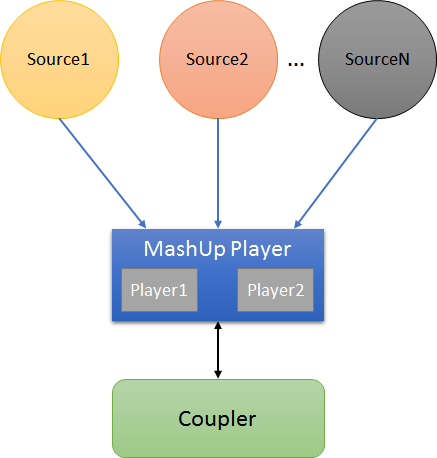
\includegraphics[scale=0.6] {figures/arqchitecture}}
	\caption{LiveSync Model}
	\label{live_arq}
\end{figure}

\textbf{\textit{Content Providers}}

Content Providers are third-parties videos streamers platforms. There are multiple Live Video Stream applications in the market, such as YouTube Live, LiveStream, TwitCast, Twitch and Ustream. One of our objective was to allow the use of different platforms as video sources, so we maximize the number of videos for an event and allow the use of already in market platforms. A Content Provider needs two requisites to be compatible with LiveSync: a Remote Player and Uptime Support. As each stream platform uses their own protocols, we opt to use their embeddable players into a MashUp application. These players must allow us to play, pause and stop the video stream. The second requisite, Uptime Support, is necessary to find the couplers among the videos. Uptime is the time passed since the beginning of the live stream until the video part being presented in the player at the moment of the call.

\textbf{\textit{Coupler}}

The Coupler is responsible for storage, distribution and calculation of synchronization points among video streams from the Content Providers.

A coupler is composed of a DAL instance and Log files. This goes in direction of the Serverless Architecture. We wanted an architecture that needed low resources (another justification for using third party stream services) and easy deployment. All that is necessary do execute the coupler is a NODE.JS (https://nodejs.org/en/) server instance. This is possible because the Coupler is fully developed in JavaScript and compatible with the HTML5 standards. To deploy the Coupler, we use a Backend as a Service or ”BaaS” platform, more specifically we use the Heroku (www.heroku.com) one, that permits free use of NODE.JS instances.

It stores synchronization information only during the duration of the event, so its stance is finished with the end of the videos and all data is lost. In the current scope, the sync info is only necessary during the event, after it, there is no need to store the information. For reasons of testing and using the filmed videos from YouTube we create log files that contains all contributions made by the crowd. If it is important to maintain all contributions and data for post analyses and further use, unstable version of the LiveSync is being configured to use a fully transactional database. We use a fully transactional database because we want to maintain track of all contributions made by the crowd, an important aspect in crowdsourcing and that is also supported by the DAL.

\textbf{\textit{MashUp Player}}

Mashups are applications generated by combining content, presentation or other applications functionalities from disparate sources. They aim to combine these sources to create useful new applications or services (the offer and consumption of data between two devices) to users. In LiveSync we combine videos coming from different sources and platforms with the synchronization information from the coupler to reproduce a synchronous presentation of these videos.

The MashUp Player (Figure~\ref{live_tvs}) is responsible for both presenting video synchronously and collecting the synchronization. Figure~\ref{live_tvs} represents the interface of the MashUp during a test: two cameras live streaming (content providers) a simulated television event to our mashup application.

\begin{figure}[h]
	\centerline{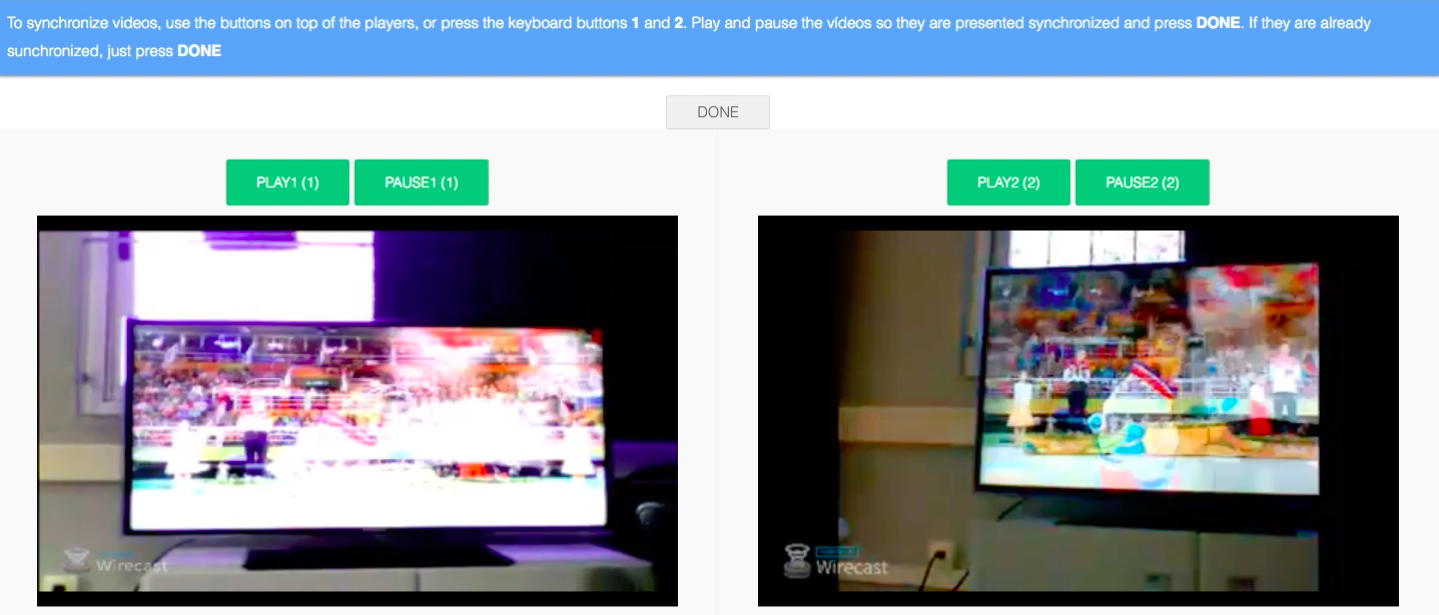
\includegraphics[scale=0.2] {figures/screen}}
	\caption{Live Streams from Olympic Games Synchronized through two different cameras}
	\label{live_tvs}
\end{figure}

On the top we have all information necessary to the user. He can aggregate new videos using the ADD NEW VIDEO options, SYNCHRONIZE the videos if he thinks the videos are not synchronized or he can just select the videos he want to watch. When just playing two selected videos from the videos list, each video player creates an instance for the player that is compatible with that source (YouTube or WebSocket). It is invisible to the user where the video is coming from.

When the user adds a video, an input text is shown to him, and he can add the video URI (WebSocket) or video ID YouTube). The page reloads and the new video is listed in the video list for everyone that connects to the application. When the video is added by the user, an message is sent to the Coupler, containing the action to add a new asset to the DAL, and the specification of it, such as label and URI.

The last functionality of the MashUp is to synchronize the videos. When the user clicks on SYNCHRONIZE, a new mode of the application is revelled showing the synchronization tools. We use a Play ’n Pause approach to synchronize the videos. After the user thinks the videos are synchronized, clicking the DONE button, his contribution is sent to the Coupler and stored in the DAL for further processing of the relation.

\subsection{Crowd Simulated DAL}
In order to validate the DAL it was designed a way to simulate a crowd, that allows us to run multiple experiments with large datasets in a viable time and without the possible biasing issues that can occur when using a human crowd. The solution found was to create the Crowd Simulator, a parameterized system that can simulate crowds with different levels of reliability, providing many contributions in short time.

To determine how the Crowd Simulator should work, we had to understand the behavior of the crowd. Yu et al.\cite{yu2012challenges} classify the crowd in four categories: Hon workers: honest worker agents who return high quality HIT (human intelligence task) results randomly 90\% of the time; MH workers: moderately honest worker agents who return high quality HIT results randomly 70\% of the time; MM workers: moderately malicious worker agents who return high quality HIT results randomly 30\% of the time; Mal workers: malicious worker agents who return high quality HIT results randomly 10\% of the time. In our scenario we consider a high quality HIT as a positive synchronization point identification or correct negation.

Per these definitions, the Crowd Simulator is settled with the percentage of honest workers in the simulated crowd, and we name this parameter as Crowd Trustworthy Degree. Each time the simulator is called, it determines the current worker reliability as so the chance of his contribution represents a high quality answer. As the objective of this experiment is validating de DAL, each high quality result is extracted from a Gold Standard Table that contains all relations between videos in dataset.

For this experiment we used the Climbing video dataset \cite{hal-01162603} that contains 89 videos captured from several different devices and users in order to register a climbing activity by distinct points of view. This climbing event has 4327.3 seconds long, and the videos starts in different offsets with durations varying between 18.96 and 1259.06 seconds. We made tests for 11 Crowd Trustworthy Degrees (from 100\% to 0\%) running 30 full simulations for each degree. Table 1 presents, for each Crowd Trustworthy Degree, the median of how many contributions were needed to converge the DAL (find all time offsets) after 30 roll of the simulation, the number of relations found, and the error rate.

As the dataset contains 89 videos, the goal was to find all 3916 relations for all pairs of videos in it. To reduce the false convergences, we used the convergence level three to determine that a value is assumed correct, this means that at least three sequential agreements are necessary to converge a value.

We also created a Gold Standard DAL built with 100\% of correct answers from de Gold Standard Table (available with the dataset), allowing us to compare the DAL generated in each run with the Gold Standard DAL for accuracy and efficiency of the simulated crowd.  Table~\ref{xp1} shows the results of the simulation. Each line corresponds to a test with different Trustworthy Degrees (reliability).  Besides the reliability, each line presents the number of necessary contributions to converge, the total amount of possible relations (not all relations will present values, as there may be GAPs among videos) found among pairs of videos and the error degree.


\begin{table}
\begin{center}
\caption{Median for all 89 Videos, after 30 rolls of simulations for each Trustworthy degree} \label{xp1}
\begin{tabular}{|c|c|c|c|}
  \hline
  Reliability & Contributions & Relations & Error
  \\
  \hline
  100\% & 11161 & 1115 & 9\% \\
  90\%  & 12101 & 1095 & 10\% \\
  80\%  & 13199 & 1095 & 10\% \\
  70\%  & 14475 & 1082 & 12\% \\
  60\%  & 16077 & 1069 & 12\% \\
  50\%  & 18015 & 1056 & 13\% \\
  40\%  & 20500 & 1052 & 14\%\\
  30\%  & 23904 & 1040 & 15\% \\
  20\%  & 28404 & 1038 & 15\% \\
  10\%  & 35121 & 1002 & 18\% \\
  0\%   & 46356 & 975  & 21\% \\
  \hline
\end{tabular}
\end{center}
\end{table}

Analyzing the result, we can see that the number of relations found don’t decrease significantly when the reliability of the crowd declines, also the percentage of the wrong relations found don’t raises dramatically. The major change among the different reliability degrees is on the number of necessary contributions to converge a DAL.

As can be seen in Figure~\ref{results-line}, between Crowd Trustworthy Degree 100\% and 50\% the results decrease linearly, below 50\% the result quality decline faster.

\begin{figure}[h]
	\centerline{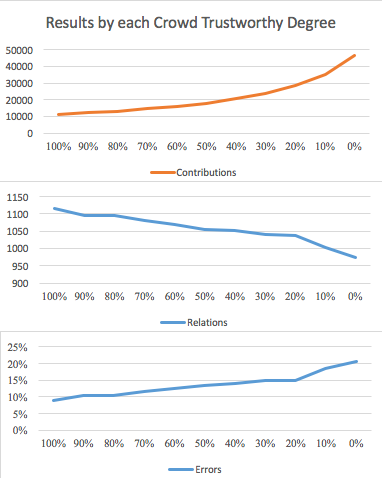
\includegraphics[scale=0.8] {figures/results-line}}
	\caption{evolution of results by each between Crowd Trustworthy Degree}
	\label{results-line}
\end{figure}



\subsection{UGV Dataset Synchronization} 
Instead of discarding the human factor, this experiment aims at testing if the human factor is able to find and synchronize an User Generated Video dataset. The Climbing video dataset \cite{hal-01162603} presents multiple videos filmed by a group during a climbing activity. The automatic technique presented with the dataset presents some limitations making this dataset ideal to test the crowd approach, so we selected part of the dataset (9 videos) to our experiment. The automatic method could identify 23\% of all pairs of videos that temporally overlap, the pairwise alignment score (PAS).

To execute our experiment, we developed the technique described in section~\ref{chunk-sync}, where the crowd member analyse video chunks (5s) pair by pair, identifying if there is relation and the precision of the relation if one exists. This was the chosen solution because requires less effort from the crowdworkers, and more detailed tests are necessary to evaluate the Frame Synchronization one, as a more complex task may compromise the worker activity.

From the known ground-truth we analysed the values resulted from the crowd to evaluate the alignment within a tolerance of 0.5s \cite{hal-01162603}. The comparison with the ground truth resulted in 88\% (PAS) of correct relations among the videos. The nine videos generated 278 chunks of video (a total of 1390 seconds to be synchronized) demanding a total of 1051 contributions. Most of these (99\%) contributions were negative ones, in other words, the crowd worker could not identify synchronization  point. This indicates that most of the crowd effort is being done in discarding synchronization point, and not really finding them.

Figure~\ref{interface} shows an instant where overlapping occurs in videos recorded using 6 different cameras are synchronously presented after the crowd contributions. The other three ones are not shown because in this instant no overlapping was indicated by the crowd. It is possible to notice how heterogeneous are the camera shots. 

\begin{figure}[h]
	\centerline{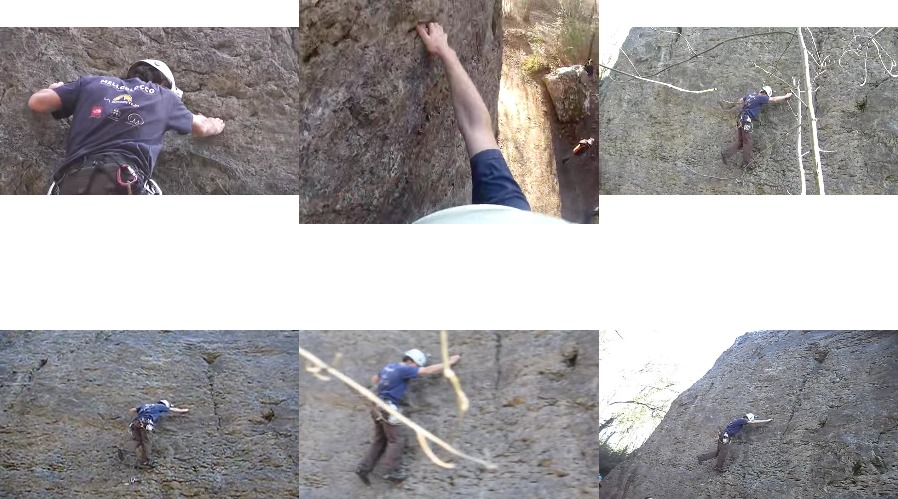
\includegraphics[scale=0.2] {figure/matrix}}
	\caption{Synchronized Video Matrix}
	\label{interface}
\end{figure}


%Considerações finais
\section{Final Remarks}

Crowds can be used in the most diverse situations: from designing a product to digitizing a word, going through most diverse scenarios, as discovering the structure of a protein. Exploring this variety of uses of the crowd this paper presented the possibility of using crowds in the video synchronization process. Using the crowd allows to address challenges that automatic processing techniques struggle to solve, like: moving cameras, constantly changing backgrounds, disappearing objects and others. A human can handle this problems without affecting his perception about a video

Nevertheless, using crowdsourcing techniques also introduces new problems to the process: which pair of videos will be sent to each user? Where are the contributions stored? How can the contributions be validated? How to know that all videos are synchronized? What are the time offsets among the videos? Do I need to compare all videos? As solution to these problems the DAL was described. An structure that can manage temporal relations and crowd contributions.

The first experiment showed the simpler where the crowd can be used: the live one. It is said simpler because the crowd has a smaller search area to find the videos alignment point. With the LiveSync this scenario can be solved and multiple mashups applications developed. The Second experiment showed us that the more reliable the crowd is, the less contributions we need and that 100\% to 60\% may generate similar results. Also we don't need the crowd to find all values: most of the relations we can infer from others. The third experiment showed us that it is possible to use the power of the crowd to synchronize video datasets, in the a hard dataset that presented challenge even to automatic solutions. From the second experiment we also learned that most contributions are to find that two chunks don't have a synchronization point. This is important and is the key point to the next steps in the development of our research, as we are developing new interfaces that helps the crowd members in identifying the synchronization points in entire videos at once, not only chunks. This will lead us in reducing the number of required contributions and achieve more accurate results.

All code involved in our research is opensource and is available in [Removed for Blind Review].



\bibliographystyle{ACM-Reference-Format}
\bibliography{sigproc} 

\end{document}
